%=============================================================================
%  CSE 465 Project Report, North South University
%  IEEE conference format, matching the faculty sample (conference_101719).
%  Compile in Overleaf with pdfLaTeX. Run TWICE so references resolve.
%  Needs: figures/fig3_main_result.png
%         figures/fig4_truncation.png
%         figures/fig5_lengths.png
%=============================================================================
\documentclass[conference]{IEEEtran}
\IEEEoverridecommandlockouts
\usepackage{cite}
\usepackage{amsmath,amssymb,amsfonts}
\usepackage{graphicx}
\usepackage{textcomp}
\usepackage{xcolor}
\usepackage{booktabs}
\usepackage{array}
\usepackage{url}
\usepackage{tikz}
\usetikzlibrary{arrows.meta,positioning,calc}

\newcolumntype{L}[1]{>{\raggedright\arraybackslash}p{#1}}

\begin{document}

\title{Reasoning Termination, Not Reasoning Capability,\\
Bounds Small Language Model Performance on\\
Competition Mathematics\\
{\footnotesize A budget forcing study of VibeThinker-3B on AIME 2025}
}

\author{\IEEEauthorblockN{Abu Ahmad}
\IEEEauthorblockA{\textit{Department of Electrical and Computer Engineering} \\
\textit{North South University}\\
Dhaka, Bangladesh \\
ID 2121725042}
\thanks{Code, measured result files and all 120 reasoning traces are available at
\protect\url{https://github.com/abuahmad369/llm-budget-forcing}. A public write up
with an interactive explorer is at
\protect\url{https://abuahmad369.github.io/reasoning-termination/}.}
}

\maketitle

%=============================================================================
\begin{abstract}
Compact reasoning models trained with reinforcement learning now report
accuracies on competition mathematics that until recently belonged to models a
hundred times larger. Those accuracies come from runs where the generation
length is effectively unlimited, and nobody reports what a realistic limit
costs. This paper measures it. A three billion parameter model was evaluated on
the 30 problems of the 2025 American Invitational Mathematics Examination, four
samples per problem, at generation budgets from one thousand to thirty two
thousand tokens, with the weights left untouched throughout. For every sample
the harness recorded not only whether the answer was right but why generation
stopped. Those turn out to be nearly the same question. Samples that reached a
natural stopping point were almost always correct. Samples cut off by the budget
scored zero, and they scored zero because no answer had been written down rather
than because a wrong one had. Appending a short phrase that closes the reasoning
segment and asks for the answer recovered between 7 and 13 accuracy points
depending on the budget, and across 139 interventions it never turned a correct
answer into an incorrect one. Three different phrasings performed identically,
which suggests the wording carries no weight and the act of stopping carries
all of it. The conclusion is awkward for current practice. A benchmark that
caps generation on a model of this kind is measuring stopping behaviour along
with reasoning ability, and reporting the sum as reasoning ability alone.
\end{abstract}

\begin{IEEEkeywords}
large language models, mathematical reasoning, test time scaling, budget forcing,
inference efficiency, benchmark evaluation
\end{IEEEkeywords}

%=============================================================================
\section{Introduction}

Language models that reason at length before answering are a recent development,
and the mechanism behind them is simpler than the results suggest. DeepSeek-R1
\cite{deepseekr1} showed that a model can be trained to reason by rewarding it
only for arriving at a checkable answer, with no supervision of the intermediate
steps at all. The optimisation behind it, group relative policy optimisation,
came from DeepSeekMath \cite{deepseekmath} and scores a group of sampled
answers against each other, using the group mean where an ordinary policy
gradient method would need a learned value function. What
falls out of this training is a model that writes a very long internal monologue,
explores an approach, abandons it, tries another, checks its arithmetic, and only
then commits to a result. The monologue is not decoration. It is where the work
happens.

VibeThinker-3B \cite{vibethinker} takes that recipe down to three billion
parameters. It is built on Qwen2.5-Coder-3B \cite{qwen25coder} and reports 91.4
percent on AIME 2025, which places it alongside models several orders of
magnitude larger. I find the size more interesting than the score. Three billion
parameters in float16 is about six gigabytes of weights, which fits on a single
consumer graphics card, and that changes who is allowed to do this kind of work.
A student in Dhaka with a free Kaggle account can run the same model the paper
reports on. That is the real argument for compact reasoning models, and it is a
good one.

There is a catch in it, and it is the reason for this paper. The published score
comes from a run with no meaningful length limit; the model card recommends a
maximum of 40,960 tokens. Generating forty thousand tokens for a single problem
is not fast on the hardware a student actually has. So the accessibility claim
rests on an assumption nobody has tested, which is that the model still performs
when you cannot afford to let it think for that long.

Cutting the budget lowers accuracy. Anyone would predict that. The question is
what was lost, and there are two possibilities that look identical in an accuracy
table and call for completely different responses. Either the model genuinely
needed those tokens to reach the answer, in which case the loss is a failure of
capability and the only fix is a better model, or it reached the answer early and
carried on verifying until the budget ran out, in which case the loss is a
failure of termination and can be repaired at inference time for almost nothing.
The two are distinguishable by measurement, and telling them apart is what this
work does. Three constraints shaped how. The weights are never modified. Every
experiment fits inside a free tier allowance of thirty GPU hours per week. And
every number reported below was measured on that hardware. None of them are
quoted from elsewhere.

The contributions of this work are as follows.

\begin{itemize}

\item A diagnosis. At the largest budget the number of correct samples per
problem equals the number that terminated naturally, problem by problem. Of 120
samples, 95 terminated and 97 were correct; of the 25 that were cut off, 23 had
written no answer at all and scored zero on that account. The whole gap between the published 91.4 percent and the 80.8 percent
measured here is a truncation artifact.

\item An intervention. Budget forcing \cite{s1}, measured on a compact model at
four budgets, gaining 7.5 to 13.3 points, significant at every budget where the
paired test could be applied, and strictly non destructive: across 139
interventions it destroyed zero correct answers.

\item A negative result. Three different forcing phrasings are statistically
indistinguishable, and a two stage variant that first asks the model to summarise
what it has established costs 2.1 times more compute for no gain. What matters is
that the model is made to commit, not how politely it is asked.

\item Upper bounds. At the smaller budgets a single forced sample beats the best
of four unforced ones, so forcing exceeds the ceiling of any method that only
selects among answers the model has already produced. Measured against the
population it could in principle recover, it captures about 80 percent.

\item The method that made the study affordable. Generation is autoregressive and
the model has no knowledge of its own budget, so the first $N$ tokens of a long
run are what a run limited to $N$ tokens would have produced. Generating once at
the largest budget therefore lets every smaller budget be scored on a CPU at no
GPU cost. It is checked experimentally in Section IV.

\end{itemize}

Section II reviews reinforcement learning for verifiable reasoning, the existing
family of inference time methods, and where budget forcing sits among them.
Section III sets out the formulation, the intervention and the statistical
procedure. Section IV describes the model, the hardware and the protocol,
including two checks on the harness itself. Section V reports the measurements
and Section VI argues about what they mean. Section VII concludes and states the
limitations plainly.

%=============================================================================
\section{Background Work and Literature Review}

\subsection{Reinforcement learning for verifiable reasoning}

The training signal behind current reasoning models is unusually crude, and that
is the point. DeepSeek-R1 \cite{deepseekr1} rewards the model when its final
answer matches a reference and says nothing about the path taken to get there.
No human labels the intermediate steps, no separate model scores them. Group
relative policy optimisation \cite{deepseekmath} makes this practical by sampling
a group of completions for the same prompt and using the group mean as the
baseline, which removes the value network that ordinary policy gradient methods
need. Long horizon reasoning is not designed into either method. It emerges,
because checking your own work turns out to raise the probability of a correct
final answer, and the reward notices.

VibeThinker-3B \cite{vibethinker} applies the same idea in the small model
regime and reports competition level mathematics accuracy at three billion
parameters. Two details in that paper matter more here than the headline number.
The first is that their evaluation imposes no output length cap. The second is
that the weakness they report falls on knowledge heavy tasks and not on
reasoning procedure, which tells you the model knows how to work through a
problem even where it lacks the facts. Neither the paper nor the model card
reports how accuracy behaves when the output length is constrained. That is the
regime anybody working on modest hardware occupies from the first day, and it is
undocumented.

\subsection{Inference time scaling}

Several methods improve accuracy without touching the weights. Self consistency
\cite{selfconsistency} samples several reasoning chains and returns the majority
answer, on the reasoning that a correct derivation can be reached by many routes
while errors scatter. Self refinement \cite{selfrefine} has the model criticise
its own output and revise it, iterating until the critique is satisfied. The
VibeThinker paper describes a related idea it calls Claim Level Reliability
Assessment, in which the model scores the reliability of individual claims inside
its own reasoning.

All three share a structural property that turns out to be decisive here. Each
one selects among, or edits, candidate answers that the model has already
produced, so the accuracy any of them can reach is bounded above by pass@$k$, the
probability that at least one of the $k$ samples is right. Where the samples all
agree, there is nothing to select between. Where the samples contain no answer at
all, there is nothing to select from. I began this project intending to build on
exactly these methods and abandoned that plan after the first baseline, for a
reason given in Section V: on this model and this benchmark, only one of thirty
problems produced samples that disagreed with each other. The bound is not
theoretical. It binds.

\subsection{Budget forcing}

Muennighoff et al. \cite{s1} introduced budget forcing as part of s1. When
generation reaches a chosen token budget, a fixed phrase is appended that closes
the reasoning segment and demands a final answer, and decoding continues briefly
from there. Their use of it is mainly in the other direction, suppressing the end
of reasoning marker to make the model think for longer, and it is evaluated
together with supervised fine tuning on a curated reasoning set. Two things
follow from that. Its behaviour as a standalone recovery mechanism on a frozen
model, with no fine tuning anywhere in the pipeline, is not characterised. And
nobody has measured whether the intervention can damage an output that would
otherwise have been correct, which is the first question a practitioner would ask
before deploying it.

\subsection{The gap}

Taken together, four specific things are missing from the literature, and this
paper addresses each of them.

\begin{enumerate}
\item Published accuracies for compact reasoning models come from uncapped runs,
and the shape of the degradation curve under realistic budgets is not
characterised anywhere, even though deployment cost is the main argument for
building compact models in the first place.
\item Failure analyses report aggregate accuracy without separating a wrong
answer from an absent one. Two failure modes that call for entirely different
remedies both score zero and are therefore invisible in the usual tables.
\item Test time scaling methods are evaluated on the cases where samples
disagree, so their behaviour where samples agree, or where samples contain
nothing to select from, goes untested.
\item Budget forcing has been evaluated as a reasoning extension mechanism
alongside fine tuning rather than as a standalone recovery mechanism on a frozen
model, and no measurement exists of whether it can destroy a correct output.
\end{enumerate}

%=============================================================================
\section{Proposed Methodology}

\subsection{Problem formulation}

Let $\pi$ be the frozen policy and $q$ a problem statement. Under an unconstrained
budget the model emits $y = (y_1,\dots,y_T)$ ending in an end of sequence token,
and an answer $a(y)$ is parsed from the final boxed expression. Under a budget $B$
the generation is cut at $\min(T,B)$ tokens. Define the termination indicator

\begin{equation}
\tau_B(y) =
\begin{cases}
1, & T \le B \\
0, & T > B
\end{cases}
\label{eq:tau}
\end{equation}

and the correctness indicator
$c_B(y) = \mathbb{1}[\,a(y_{1:\min(T,B)}) = a^{\star}\,]$, where $a^{\star}$ is
the ground truth.

Writing the two indicators separately is what makes the competing explanations
testable, because they predict different joint behaviour. If the accuracy loss is
a capability failure, then a truncated trace is wrong because the reasoning inside
it is incomplete, and correctness should fall gradually and in much the same way
whether or not a trace happened to terminate. If instead it is a termination
failure, correctness should be close to total among terminated samples and close
to zero among truncated ones, as written in (\ref{eq:hyp}). These are not
competing interpretations of one number. They are two different pictures, and a
harness that records why each generation stopped can simply look and see which one
it is.

\begin{equation}
\Pr[c_B = 1 \mid \tau_B = 1] \approx 1, \quad
\Pr[c_B = 1 \mid \tau_B = 0] \approx 0
\label{eq:hyp}
\end{equation}

\subsection{Budget forcing}

The intervention acts on truncated samples and on nothing else. Take the prefix
that the budget cut short, append a fixed phrase $\phi$ that closes the reasoning
block and asks for a final answer, and decode greedily for a short continuation,
as in (\ref{eq:forcing}). Samples that reached an end of sequence token on their
own are left exactly as they were, never re read and never re decoded. That
restriction is the reason the method cannot lower the score: an answer the model
already committed to is never given the opportunity to change. The cost is small
enough to state precisely, since the continuation is about five generated tokens
per intervened sample.

\begin{equation}
\hat{a} = a\!\left(\pi\!\left(q \oplus y_{1:B} \oplus \phi\right)\right)
\label{eq:forcing}
\end{equation}

Three phrasings were measured instead of one, because a single phrasing that
worked would leave open the objection that the gain came from prompt engineering
and not from the act of stopping. $V_1$ is a bare demand, closing the
reasoning tag with \texttt{\textless/think\textgreater} and continuing ``I have
reasoned enough. Based on the work above, the final answer is'' followed by an
open boxed expression; $V_3$ is a soft deadline that warns the model it has little
space left before making the same demand; and $V_2$ is a two stage variant in
which the model is first asked to summarise what it has established and only then
asked for the answer.

\subsection{Prefix consistency}

Sweeping eleven budgets by running eleven separate generations would have cost
more GPU time than the whole allowance, and it is unnecessary. The model decodes
left to right, one token conditioned on those before it, and it has no
representation of how much budget remains; nothing in the forward pass depends on
where generation is going to be stopped. So the distribution over the first $N$
tokens is the same whether the run was going to end at $N$ or at some larger $B$,
which is the identity in (\ref{eq:prefix}). The practical consequence
is worth stating plainly. Generate once at the largest budget, store the full
trace, and every smaller budget becomes a slice of a string that a CPU can cut for
free. This is an empirical claim about the implementation as much as a
mathematical one, so Section IV tests it directly instead of assuming it.

\begin{equation}
y_{1:N} \Big|_{\text{budget } N}
\;\overset{d}{=}\;
\left(y \Big|_{\text{budget } B}\right)_{1:N},
\quad N \le B
\label{eq:prefix}
\end{equation}

\subsection{Statistical procedure}

The same samples are scored twice, once before the intervention and once after,
so the design is paired and an unpaired test would throw away the pairing and
answer a question nobody asked. McNemar's test with a continuity correction
\cite{mcnemar} is the right tool, and it is given in (\ref{eq:mcnemar}), where $b$
counts samples that changed from incorrect to correct and $c$ counts the reverse.
Only the discordant pairs carry information, which is why the samples that were
already correct do not appear in the statistic. The quantity $c$ is interesting on
its own, separately from the test, because it is a direct count of how often the
intervention destroyed a correct answer. Wilson score intervals \cite{wilson} are
used for the ceiling proportions in Section V, since those denominators are small
enough that a normal approximation would give intervals running past the ends of
the scale.

\begin{equation}
\chi^{2} = \frac{\left(|b - c| - 1\right)^{2}}{b + c}
\label{eq:mcnemar}
\end{equation}

\subsection{System design}

Fig. \ref{fig:pipeline} shows how the pieces fit together. Generation runs once,
at the largest budget, and is the only expensive stage. Every smaller budget is
produced by truncating the stored traces on a CPU and scoring the result, which
costs nothing and can be repeated as often as needed. Only the samples that came
back truncated go back to the GPU, and only for the few tokens that the forcing
step generates.

\begin{figure*}[t]
\centering
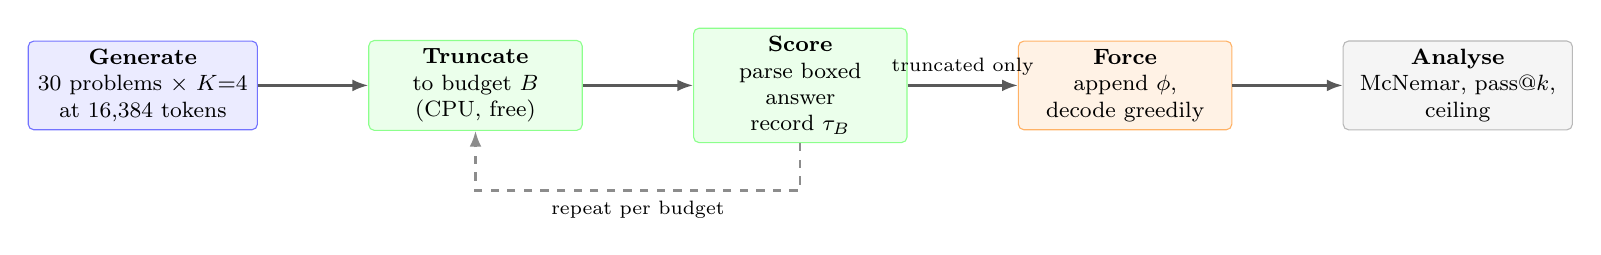
\begin{tikzpicture}[
  node distance=7mm,
  box/.style={draw,rounded corners=2pt,align=center,minimum height=10mm,
              inner sep=3pt,font=\footnotesize},
  gen/.style={box,fill=blue!8,draw=blue!55,text width=27mm},
  cpu/.style={box,fill=green!8,draw=green!45,text width=25mm},
  gpu/.style={box,fill=orange!10,draw=orange!60,text width=25mm},
  ana/.style={box,fill=gray!8,draw=gray!55,text width=27mm},
  ar/.style={-{Latex[length=2mm]},thick,draw=black!65}
]
\node[gen] (gen) {\textbf{Generate}\\30 problems $\times$ $K{=}4$\\at 16{,}384 tokens};
\node[cpu, right=14mm of gen] (trunc) {\textbf{Truncate}\\to budget $B$\\(CPU, free)};
\node[cpu, right=14mm of trunc] (score) {\textbf{Score}\\parse boxed answer\\record $\tau_B$};
\node[gpu, right=14mm of score] (force) {\textbf{Force}\\append $\phi$,\\decode greedily};
\node[ana, right=14mm of force] (stats) {\textbf{Analyse}\\McNemar, pass@$k$,\\ceiling};

\draw[ar] (gen) -- (trunc);
\draw[ar] (trunc) -- (score);
\draw[ar] (score) -- node[above,font=\scriptsize]{truncated only} (force);
\draw[ar] (force) -- (stats);
\draw[ar,dashed,draw=black!45] (score.south) -- ++(0,-6mm) -| (trunc.south)
      node[below,font=\scriptsize,pos=0.25]{repeat per budget};
\end{tikzpicture}
\caption{Experimental pipeline. Generation runs once at the largest budget.
Smaller budgets come from truncating the stored traces on a CPU, which costs
nothing. Only the forcing step returns to the GPU, and it acts on truncated
samples alone.}
\label{fig:pipeline}
\end{figure*}

%=============================================================================
\section{Experiments}

\subsection{Model, dataset and hardware}

The subject model is VibeThinker-3B, used exactly as published, with the weights
never modified at any point in the study. The benchmark is the 30 problem AIME
2025 set as distributed in \texttt{math-ai/aime25}. A reader will reasonably ask
why a 2025 examination is being used in 2026, so I will answer it before it is
asked: AIME 2026 has no public dataset, and running on AIME 2025 has a
compensating advantage, since VibeThinker's own paper reports a number for that
exact set and so the harness can be checked against a published figure before any
new claim is made. Every answer on this examination is an integer between 0 and
999, which means correctness is decided by exact match against a reference number
with no judge model and no grading rubric anywhere in the loop.

The inference engine was chosen on measured throughput. A
first throughput probe with HuggingFace \texttt{transformers} gave 15.2 tokens per
second, which projected to well over a hundred GPU hours for the planned sweep and
killed the original experimental design outright. vLLM \cite{vllm} raised the same
workload on the same card to 31.4 tokens per second at $K{=}1$, 145.9 at $K{=}8$
and 246.4 at $K{=}32$, a 16.2 times improvement, through continuous batching and
by sharing the prefix cache across samples drawn from a common prompt. Sampling
many completions from one prompt is close to the best case for that engine, which
is why the gain is so large here. Table \ref{tab:tools} lists each component and
why it was selected.

\begin{table*}[t]
\caption{Software and Hardware Components}
\label{tab:tools}
\centering
\footnotesize
\begin{tabular}{@{}L{2.4cm}L{3.4cm}L{3.4cm}L{6.4cm}@{}}
\toprule
\textbf{Tool} & \textbf{Function} & \textbf{Alternatives} & \textbf{Reason selected} \\
\midrule
vLLM & Inference engine & HF \texttt{transformers}, TensorRT-LLM &
$16.2\times$ faster through continuous batching and prefix sharing; the workload
is many samples from one prompt, its best case \\
\addlinespace
Tesla T4, 16\,GB & Accelerator & A100, TPU v4 & The only hardware on the free
tier; forces \texttt{float16} and rules out FlashAttention-2 \\
\addlinespace
VibeThinker-3B & Subject model & Qwen3-4B, Phi-4-mini & Frontier accuracy at 3B; a
published AIME 2025 score allows harness validation \\
\addlinespace
\texttt{math-ai/aime25} & Benchmark & AIME 2024, HMMT & Integer answers allow
exact matching against a published reference number \\
\addlinespace
Kaggle Notebooks & Compute platform & Colab, Lambda Labs & 30 GPU hours per week
at no cost; batch execution survives disconnection \\
\bottomrule
\end{tabular}
\end{table*}

The card is a Tesla T4 with 15.64 GB of usable memory and compute capability 7.5,
and three consequences of that follow the experiment everywhere. FlashAttention-2
requires compute capability 8.0 or above, so vLLM falls back to a Triton attention
backend. bfloat16 is not supported on Turing, so float16 is mandatory here and
not a choice. And the key value cache holds 192,272 tokens at 90 percent memory
utilisation, which fixes how many samples can be in flight at once through
(\ref{eq:conc}). That last one is why throughput is not a single number for this
model: a 32k context window leaves room for roughly six concurrent sequences and
sustained 60 to 71 tokens per second, while an 8k window leaves room for
twenty three and sustained 246.

\begin{equation}
\text{concurrency} = \frac{192{,}272}{\texttt{max\_model\_len}}
\label{eq:conc}
\end{equation}

\subsection{Protocol}

Decoding parameters are frozen across every arm of the experiment: temperature
1.0, a top p value of 0.95, seed 0, and $K = 4$ samples per problem, giving 120
samples per condition. Prompts come from the model's own chat template rather
than from a hand written wrapper. Answers are extracted by finding the final
boxed expression with a brace depth parser, so that a nested expression inside the
box is captured whole. One implementation of the prompt builder, the parser and
the forcing phrase is shared by every script in the study, which matters more than
it sounds: with separate copies, a change made while debugging one arm can silently
apply to one condition and not another, and the resulting difference looks like a
finding. Budgets of 4,096, 8,192, 16,384 and 32,768 tokens were used for the
forcing experiments, with the finer sweep in Section V taken from stored traces.

The part of the protocol that does the real work is the termination log. For every
sample the harness records why generation stopped, which separates a sample that
produced a wrong answer from one that produced no answer at all. Without that
field, (\ref{eq:hyp}) cannot be tested, because both failure modes appear in an
accuracy table as the same zero. This is a small change to a standard evaluation
loop, and it is the difference between reporting that accuracy fell and being able
to say why.

\subsection{Compute expenditure}

\begin{table}[t]
\caption{Measured Compute Expenditure}
\label{tab:compute}
\centering
\footnotesize
\begin{tabular}{@{}L{3.1cm}rL{3.4cm}@{}}
\toprule
\textbf{Stage} & \textbf{GPU h} & \textbf{Purpose} \\
\midrule
Setup and probes & 1.50 & Environment audit, throughput \\
Baseline, 32K & 8.87 & 30 problems, $K{=}4$ \\
Forcing, 4K and 8K & 2.06 & First forcing measurement \\
Forcing variants, 16K & 8.89 & Traces and six forcing passes \\
Trace analysis & 0.00 & CPU only; curve and figures \\
Paired analysis & 1.28 & McNemar at 8K and 16K \\
Upper bounds & 0.00 & CPU only; pass@$k$, ceiling \\
\midrule
\textbf{Total} & \textbf{22.60} & \\
\bottomrule
\end{tabular}
\end{table}

\subsection{Harness validation}

Two checks were run before any of the results in Section V were believed. The
first compares the unconstrained baseline against the published figure. Running
the model at a 32K budget reproduced 80.8 percent against the 91.4 percent
reported in \cite{vibethinker}. The direction of that discrepancy is worth saying
out loud, because a reproduction that comes in above a published number invites a
contamination argument and this one comes in below it. Section V explains the
shortfall, and it is not a scoring error.

The second check tests the prefix consistency identity in (\ref{eq:prefix})
directly, since everything downstream of it depends on it holding. An 8,192 token
condition was measured two ways, once by a genuine run with that limit set on the
engine and once by truncating stored 16,384 token traces at the same point. The
two gave 54.2 and 55.8 percent, a difference of two samples out of 120, which is
within what temperature 1.0 sampling produces on its own. Had this check failed,
the entire budget sweep would have been an artifact of the truncation procedure
rather than a property of the model.

%=============================================================================
\section{Results}

\subsection{Termination against correctness}

\begin{table}[t]
\caption{Correct Against Naturally Terminated Samples, 32K Budget}
\label{tab:decomp}
\centering
\footnotesize
\begin{tabular}{@{}crrl@{}}
\toprule
\textbf{Problem} & \textbf{Correct} & \textbf{Terminated} & \textbf{Note} \\
\midrule
8  & 2/4 & 2/4 & \\
13 & 0/4 & 0/4 & all truncated \\
14 & 0/4 & 0/4 & all truncated \\
19 & 2/4 & 2/4 & \\
26 & 3/4 & 3/4 & \\
27 & 1/4 & 1/4 & \\
29 & 0/4 & 0/4 & all truncated \\
\midrule
21 problems & 4/4 & 4/4 & solved by all \\
\bottomrule
\end{tabular}
\end{table}

Table \ref{tab:decomp} sets the number of correct samples beside the number that
terminated naturally, problem by problem, at the 32K budget. The 21 problems the
model solved on all four samples also terminated on all four, contributing 84
samples to each column, and the seven problems listed individually match column
for column as well. That is 28 of the 30 problems matching exactly. In aggregate
there are 97 correct samples and 95 terminated ones out of 120, so the two
columns differ by two samples in total, and both of them sit in the two problems
not shown in the table. Of the 25 samples that were cut off by the budget, 23
scored zero; the other two are those same stragglers, truncated traces that
happened to contain a boxed expression before the cut. Interpretation is left to
Section VI; this subsection reports arithmetic.

\subsection{Accuracy against budget}

\begin{figure*}[t]
\centering
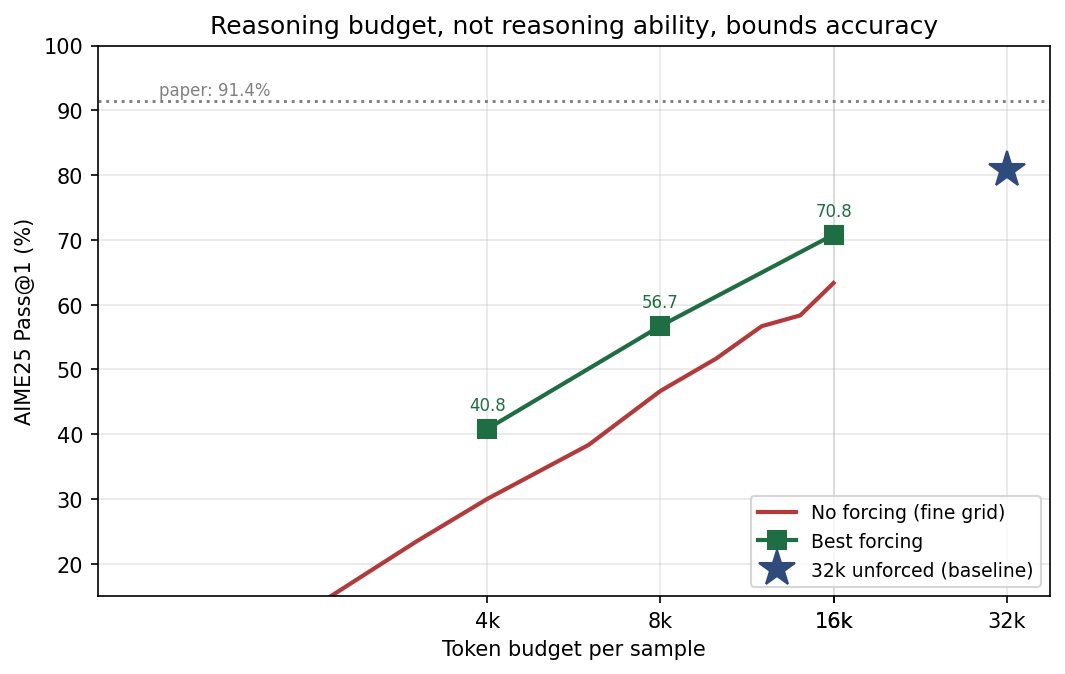
\includegraphics[width=0.82\textwidth]{figures/fig3_main_result.png}
\caption{Accuracy against generation budget, with and without budget forcing. The
dotted line marks the accuracy reported in \cite{vibethinker} under an
unconstrained budget.}
\label{fig:main}
\end{figure*}

\begin{table}[t]
\caption{Accuracy and Truncation Against Budget, No Forcing}
\label{tab:curve}
\centering
\footnotesize
\begin{tabular}{@{}rrr@{\hspace{1.4em}}rrr@{}}
\toprule
\textbf{Budget} & \textbf{Pass@1} & \textbf{Trunc.} &
\textbf{Budget} & \textbf{Pass@1} & \textbf{Trunc.} \\
\midrule
1K & 3.3\%  & 100.0\% & 8K  & 46.7\% & 67.5\% \\
2K & 13.3\% & 98.3\%  & 10K & 51.7\% & 63.3\% \\
3K & 23.3\% & 92.5\%  & 12K & 56.7\% & 59.2\% \\
4K & 30.0\% & 87.5\%  & 14K & 58.3\% & 53.3\% \\
6K & 38.3\% & 77.5\%  & 16K & 63.3\% & 48.3\% \\
\bottomrule
\end{tabular}
\end{table}

\begin{figure}[t]
\centering
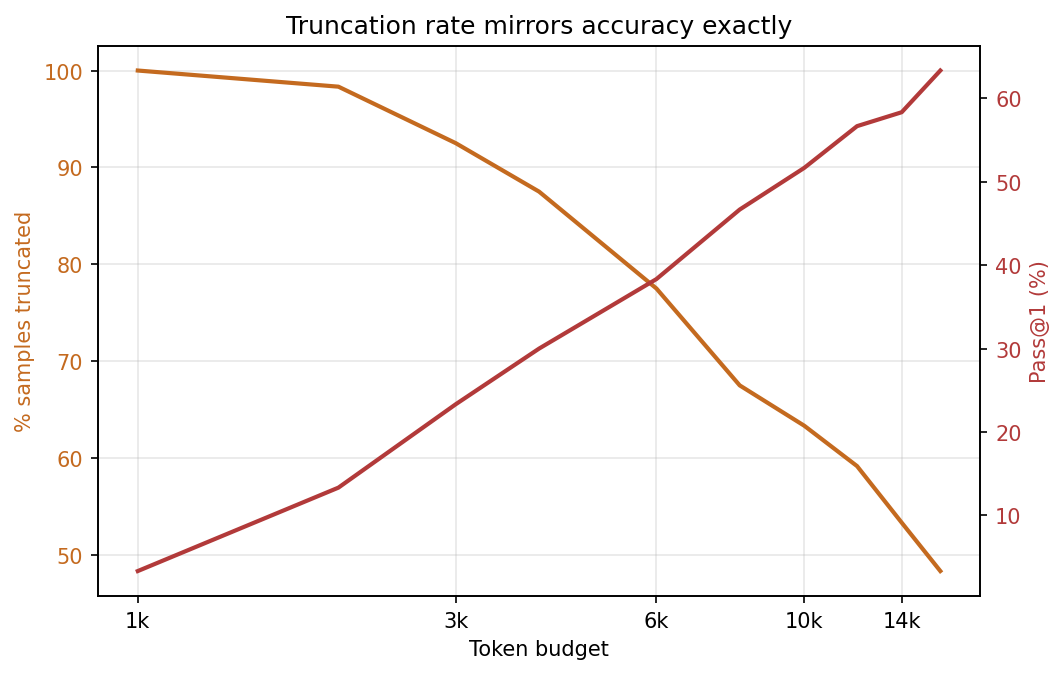
\includegraphics[width=\columnwidth]{figures/fig4_truncation.png}
\caption{Truncation rate and accuracy move inversely with budget. Left axis, the
percentage of samples cut off. Right axis, Pass@1 over the same samples.}
\label{fig:trunc}
\end{figure}

Table \ref{tab:curve} and Fig. \ref{fig:trunc} give the degradation curve. Pass@1
rises from 3.3 percent at a 1K budget to 63.3 percent at 16K and reaches 80.8
percent at 32K, while the truncation rate falls from 100 percent to 48.3 percent
and then to 20.8 percent across the same range. The two curves are close to
mirror images. One detail in the table is easy to read past and should not be:
from 3K upward, accuracy runs between about 12 and 18 points higher than the
natural termination rate, which is arithmetically impossible if an answer can only
be scored from a completed trace. The explanation is that the model sometimes
writes an intermediate boxed expression in the middle of a derivation, usually
when recording a partial result, and the parser recovers it even though the trace
never terminated. So the unforced baseline is not a clean measurement of completed
reasoning. It already includes some truncated samples that were answered by
accident, which makes it a conservative comparison point for the intervention that
follows. One further observation from the same traces: across all 1,200 sample
budget observations in the sweep, the model volunteered exactly one answer that
was wrong. When it fails under a budget, it fails silently.

\begin{figure}[t]
\centering
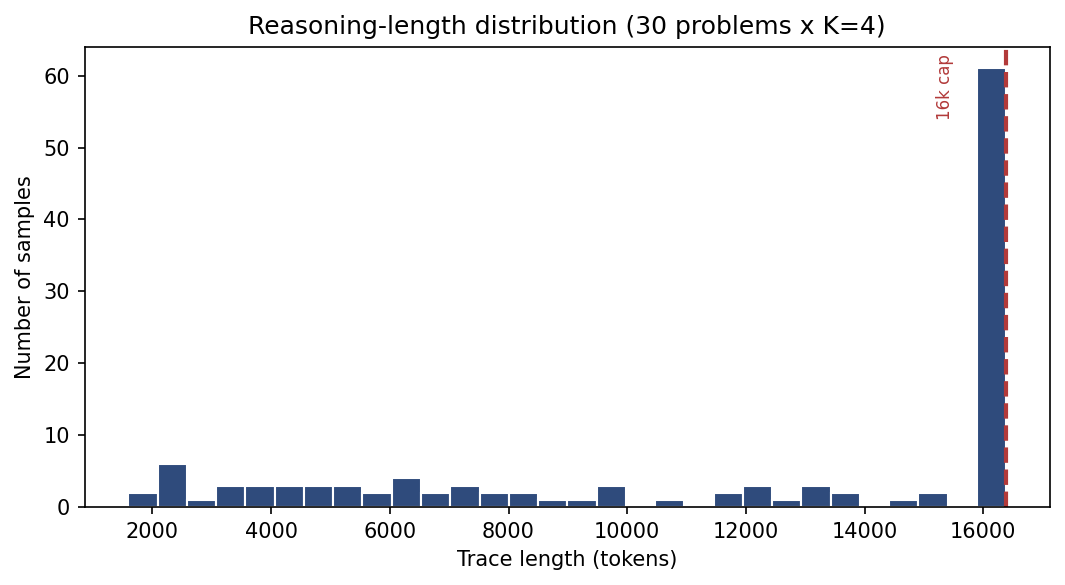
\includegraphics[width=\columnwidth]{figures/fig5_lengths.png}
\caption{Distribution of reasoning trace lengths over 30 problems and four samples
each. The distribution is right censored at 16{,}384 tokens; the mass at the cap
is an artifact of the imposed limit, not the model stopping on its own.}
\label{fig:lengths}
\end{figure}

Fig. \ref{fig:lengths} shows the trace length distribution, whose median is 15,961
tokens. The spike at the right edge is not the model's natural stopping point. It
is the imposed limit, and the distribution is right censored there, so the true
tail extends past the edge of the plot by an unknown amount.

\subsection{Effect of budget forcing}

\begin{table}[t]
\caption{Effect of Budget Forcing on AIME 2025 Pass@1}
\label{tab:main}
\centering
\footnotesize
\begin{tabular}{@{}lrrrc@{}}
\toprule
\textbf{Budget} & \textbf{No forcing} & \textbf{Forced} & \textbf{Gain} &
\textbf{McNemar $p$} \\
\midrule
4K  & 27.5 / 30.0\% & 40.8\% & $+13.3$ & not run \\
8K  & 46.7\%        & 55.8\% & $+9.1$  & $\mathbf{0.0026}$ \\
16K & 63.3\%        & 70.8\% & $+7.5$  & $\mathbf{0.0077}$ \\
32K & 80.8\%        & n/m    &         & \\
\bottomrule
\end{tabular}
\end{table}

Table \ref{tab:main} gives the headline effect. Forcing adds 13.3 points at 4K,
9.1 at 8K and 7.5 at 16K, and the gain is significant at both budgets where the
paired test was applied. The 4K row carries two baselines and the reason should be
stated and not tidied away. That budget was measured twice at different points
in the project, once by a dedicated run that gave 27.5 percent and once by
truncating stored traces, which gave 30.0 percent. Three samples out of 120
separate them, which is within sampling noise, but they came from different
experiments and so the 4K point is not plotted as part of a single series with 8K
and 16K in Fig. \ref{fig:main}. Forcing at 32K was not measured, and the cell is
marked accordingly instead of being filled by extrapolation.

\subsection{Test for harm}

\begin{table}[t]
\caption{Paired Contingency, Truncated Samples Only}
\label{tab:paired}
\centering
\footnotesize
\begin{tabular}{@{}lrrrrrr@{}}
\toprule
\textbf{Budget} & \textbf{Trunc.} & \textbf{$b$} & \textbf{$c$} &
\textbf{r$\rightarrow$r} & \textbf{$\chi^2$} & \textbf{$p$} \\
\midrule
8K  & 81 & 11 & \textbf{0} & 17 & 9.09 & 0.0026 \\
16K & 58 & 9  & \textbf{0} & 14 & 7.11 & 0.0077 \\
\bottomrule
\end{tabular}
\end{table}

Table \ref{tab:paired} gives the paired contingency over the truncated samples,
which are the only ones the intervention touches. At 8K, 81 samples were truncated
and 11 changed from incorrect to correct; at 16K, 58 were truncated and 9 changed.
In both cases $c$, the count of samples that changed from correct to incorrect, is
zero. Across all 139 interventions, not one correct answer was destroyed. The right to right column records the samples that were already correct
before forcing and remained correct after it: 17 at 8K and 14 at 16K, so 31
truncated traces already contained a correct boxed expression, and forcing
re derived the identical value in every one of the 31. Measured against the
samples it could plausibly rescue, forcing recovered 11 of 64 at 8K and 9 of 44 at
16K, rates of 17.2 and 20.5 percent, against the 0.1 percent that guessing a
uniform integer between 0 and 999 would achieve. The composition of the 120
samples changes in a way worth recording: at 8K the unforced arm produced 56
correct, no wrong answers and 64 with no answer at all, while the forced arm
produced 67 correct, 53 wrong and none missing. Forcing converts silence into
answers, most of which are wrong, and the correct ones are pure gain.

\subsection{Sensitivity to the forcing phrase}

\begin{table}[t]
\caption{Comparison of Forcing Phrasings}
\label{tab:variants}
\centering
\footnotesize
\begin{tabular}{@{}lrrr@{\hspace{1.2em}}rr@{}}
\toprule
& \multicolumn{3}{c}{\textbf{Pass@1}} & \multicolumn{2}{c}{\textbf{Cost, min}} \\
\cmidrule(lr){2-4}\cmidrule(l){5-6}
\textbf{Budget} & $V_1$ & $V_3$ & $V_2$ & $V_1$ & $V_2$ \\
\midrule
8K  & 55.8\% & 55.8\% & 56.7\% & 21.2 & 47.8 \\
16K & 70.8\% & 70.8\% & 70.8\% & 54.9 & 117.3 \\
\bottomrule
\end{tabular}
\end{table}

At 16K all three phrasings return 70.8 percent, the same figure to the sample. At
8K the two stage variant $V_2$ leads by 0.9 points, which is one sample out of
120. The wall clock cost is where they differ: $V_2$ took 47.8 minutes against
21.2 at 8K and 117.3 against 54.9 at 16K, a factor of 2.1 at both budgets.

\subsection{Upper bounds}

\begin{table}[t]
\caption{Budget Forcing Against the Selection Oracle}
\label{tab:oracle}
\centering
\footnotesize
\begin{tabular}{@{}lrr@{}}
\toprule
\textbf{Budget} & \textbf{Unforced pass@4} & \textbf{Forced pass@1} \\
\midrule
4K  & 40.0\% & \textbf{40.8\%} \\
8K  & 53.3\% & \textbf{55.8\%} \\
16K & \textbf{73.3\%} & 70.8\% \\
\bottomrule
\end{tabular}
\end{table}

\begin{table*}[t]
\caption{Extraction Ceiling on the Recoverable Population}
\label{tab:ceiling}
\centering
\footnotesize
\begin{tabular}{@{}lrrrrrrrr@{}}
\toprule
\textbf{Budget} & \textbf{Truncated} & \textbf{Already correct} &
\textbf{Rescuable} & \textbf{Has answer} & \textbf{False pos.} &
\textbf{Ceiling} & \textbf{Rescued} & \textbf{Captured} \\
\midrule
8K  & 81 & 17 & 64 & 16 & 2 & 14 & 11 & 78.6\% \\
16K & 58 & 14 & 44 & 11 & 0 & 11 &  9 & 81.8\% \\
\bottomrule
\end{tabular}
\end{table*}

Table \ref{tab:oracle} sets a single forced sample against the best of four
unforced ones, which is the accuracy an ideal selection method would reach if it
always picked the right sample out of four. At 4K and 8K the single forced sample
wins, 40.8 against 40.0 and 55.8 against 53.3. At 16K the ordering reverses and
the oracle wins, 73.3 against 70.8. The comparison is deliberately unequal and the
caveat has to travel with the number: this is forced pass@1 against unforced
pass@4, and forced pass@4 was not computed, so the table shows that forcing one
sample can beat selecting among four, not that forcing beats selection when both
are given the same sampling budget.

Table \ref{tab:ceiling} asks a narrower question. Of the truncated samples that
were not already correct, how many contain the right answer somewhere in the
trace, and how many of those does forcing actually extract? At 8K the rescuable
population is 64 samples, 16 of which mention the correct answer, and a false
positive control removes 2, leaving a ceiling of 14; forcing recovered 11, or 78.6
percent. At 16K the same procedure gives a ceiling of 11 and forcing recovered 9,
or 81.8 percent. Those denominators are 14 and 11, so the Wilson intervals are
wide, running roughly from 52 to 92 percent and from 52 to 95 percent. The false
positive control, which counts how often the target number appears in a trace by
coincidence, ran between 0 and 4.9 percent against a signal of 32 to 41 percent,
so the effect is not an artifact of string matching. The last column of the
rescuable population is the one that matters for the rest of this paper: only 16
of 64 traces at 8K, and 11 of 44 at 16K, mention the correct answer anywhere in
their final fifth.

%=============================================================================
\section{Analysis}

\subsection{Termination, not capability}

Table \ref{tab:decomp} matches column for column, and that is the whole result.
Correctness is near total among samples that terminated and near zero among
samples that did not, which is the pattern (\ref{eq:hyp}) predicts under the
termination hypothesis. The capability hypothesis predicts something visibly
different, a smooth decline across both groups as reasoning quality degrades with
less room to work, and that is not what the table shows. Nothing in between is
consistent with a column for column match on 28 of 30 problems. The gap between
the published 91.4 percent and the 80.8 percent measured at 32K is therefore a
truncation artifact rather than a reasoning deficit. Nothing in the arithmetic
strains against that reading: 23 samples scored zero purely for want of a written
answer, which is 19.2 percent of the whole sample set, against a shortfall of only
10.6 points to be explained.

Problem 1 is the clearest single case, and its answer is 588. The trace derives
$AB = 28$ and $AC = 91$, sets up coordinates for the auxiliary point, and reaches
the conclusion that the area of the heptagon equals the area of the triangle.
Somewhere in that working, the value 588 appears. It then keeps checking, re examines
the construction, and the budget expires before it ever writes a boxed answer. The
mathematics was finished and scored zero. I do not think there is a stronger way
to make the argument than that: the reasoning succeeded, and only the act of
stating the result failed.

\subsection{Why forcing cannot do harm}

The zero in the $c$ column of Table \ref{tab:paired} is not luck, and the right to
right column shows why. Thirty one truncated traces already contained a correct
boxed expression before the intervention. Forcing overwrote every one of them,
appending its phrase and asking again, and in all 31 cases the model produced the
identical value. Once a result has been established firmly enough for the model to
write it down once, being asked to write it down again reproduces it, because the
working that produced it is still sitting in the context window and the
continuation is conditioned on all of it. The intervention is not asking the model
to reconsider. It is asking it to read out.

There is a practical consequence. Early on I built a hybrid policy that checked
each truncated trace for an existing boxed answer, kept it if one was present, and
forced only when none was, on the assumption that overwriting a good answer was a
risk worth engineering around. It scores identically to plain forcing at every
budget, because the case it protects against does not occur. I removed it. The
simpler rule is not a compromise here; the extra logic was solving a problem that
the measurement says does not exist.

\subsection{Why the phrasing does not matter}

Three phrasings, one of them substantially more elaborate than the others, return
the same accuracy to within a single sample. Table \ref{tab:variants} is a
negative result and it is more informative than a positive one would have been.
If a carefully worded instruction had beaten a blunt one, the effect would have
been at least partly a prompting effect and the mechanism would be ambiguous.
Since they tie, what the intervention supplies cannot be information. It is
permission to stop. The information needed to answer is already in the trace, put
there by the model itself, and no amount of rewording the request adds to it.

The cost figures in that table need one caution attached, because they are easy to
misread as the cost of the method. They are not. Almost all of the wall clock time
is prefill, re reading a stored trace of up to sixteen thousand tokens so the
model has the context to continue from, while the forcing step itself generates
about five tokens. A deployed implementation would keep the key value cache from
the original generation and continue directly from it, at which point forcing costs
five tokens and nothing else. The 2.1 times gap between $V_1$ and $V_2$ is real and
it is a reason to prefer $V_1$, but the absolute minutes are a property of this
harness and not of budget forcing.

\subsection{What forcing can and cannot recover}

Put problem 1 next to problem 13 and the mechanism is visible. In problem 1, three
of the four summaries produced by the $V_2$ variant contain genuine derived
quantities, the side lengths and the coordinates of the auxiliary point, and
forcing yields 588, which is correct. In problem 13, whose answer is 60, the
summaries are still setting up: one of them records that the geometric median is
the unique point minimising the sum of distances, which is true, relevant and not
progress. Forcing yields 124 and 184 on two different samples, stated with the
same confidence as 588 and both wrong. The model did not derive an answer, so
forcing invented one.

That contrast generalises into a single statement: budget forcing recovers answers
that are already latent in the trace and cannot manufacture reasoning that never
happened. Every one of the four findings in this paper follows from it. The gain
is real because latent answers are common, since a model that has been trained to
verify its work will often reach a result long before it is willing to stop. The
gain is bounded because most failures are genuinely incomplete. Forcing is non
destructive because a latent answer is stable under re elicitation, which is what
the 31 identical re derivations show. And the phrasing is irrelevant because what
is being supplied is a decision to conclude rather than any content.

The same statement says where the remaining headroom is not. Only 16 of 64
rescuable traces at 8K, and 11 of 44 at 16K, mention the correct answer anywhere
near the end, so roughly three quarters of the failures never derived it. No
extraction procedure, however clever, can read out an answer that was never
written. Whatever is left to gain at these budgets is in generating the reasoning
faster, not in reading it out better.

\subsection{Implications for evaluation practice}

A benchmark that caps generation on a long horizon reasoning model is measuring a
composite of two things, how well the model reasons and how readily it stops, and
it reports that composite as reasoning ability. The two are separable, this paper
separates them, and the separation is not expensive: logging a stop reason costs
one field per sample. What makes this more than a technicality is the size of the
effect. Under a capped protocol, an intervention that appends one sentence and
generates five tokens is worth 7 to 13 points, which is larger than the margin
that separates many published systems from each other. My own view, and I hold it
after watching a model derive 588 and then score zero for not saying so, is that
truncation rate should be reported next to accuracy as a matter of routine. It
costs nothing, it makes results at different budgets comparable, and without it a
reader cannot tell whether a number reflects what the model knows or how long it
was allowed to talk.

%=============================================================================
\section{Conclusion}

This paper asked whether the accuracy a compact reasoning model loses under a
constrained generation budget reflects a failure of reasoning or a failure of
termination, and on VibeThinker-3B over AIME 2025 the two separate cleanly.
Samples that reached a natural stopping point were almost always correct. Samples
that the budget cut short scored zero, and they scored zero for want of a written
answer, not because the reasoning inside them had gone wrong. At the 32K
budget the correct count and the terminated count match problem by problem, which
is what the termination hypothesis predicts and what the capability hypothesis
does not.

Budget forcing, applied to a frozen model with nothing else changed, recovered 7.5
to 13.3 points depending on the budget, significant by McNemar's test at both
budgets where the paired design could be applied. It never converted a correct
answer into an incorrect one across 139 interventions, and in the 31 cases where
the truncated trace already held a correct answer it re derived the same value
every time. Three phrasings were statistically indistinguishable, so what the
intervention supplies is permission to conclude rather than a better instruction.
A single forced sample beat the best of four unforced samples at the two smaller
budgets, which places the method above the ceiling of any approach that only
selects among answers that already exist. Measured against the population it could
in principle recover, it captured roughly 80 percent. All of it was measured in
22.60 GPU hours on hardware that is free to anyone with an internet connection.

\subsection{Limitations}

The scope is one model, one benchmark and one seed. The intervals reported here
are binomial over 120 samples and no estimate of run to run variance was made, so
the defensible claim is that the effect exceeds plausible sampling noise, not that
it would replicate across seeds. $K = 4$ is small for a pass@$k$ analysis. The
extraction ceiling rests on populations of 11 and 14 samples, which is why its
Wilson interval spans roughly 52 to 95 percent, and that number should be read as
an order of magnitude and not as a precise measurement. AIME 2026 has no public dataset,
so AIME 2025 was used; it predates the subject publication and sat inside that
paper's evaluation scope, and no independent decontamination check was run here.
The \texttt{max\_model\_len} setting differed across arms for memory reasons and
was not controlled as a variable. The cost figures for forcing are bound to this
implementation and would fall substantially with cache reuse. Forcing at 32K and
forced pass@4 were both left unmeasured. Finally, an earlier version of the
extraction ceiling was computed and then retracted, after the denominator turned
out to coincide with the set of already correct samples, which made the numerator
and denominator disjoint and the ratio meaningless. It was recomputed against the
truncated and incorrect population, and Table \ref{tab:ceiling} reports the
corrected figure.

\subsection{Future work}

Four directions follow directly. The first is a cache reusing implementation of
forcing, which would cut its cost to roughly the five tokens it actually
generates and make it free enough to apply by default. Learned termination is the
second: since about three quarters of failures never derive the answer at all,
teaching the model to conclude sooner addresses the cause instead of the symptom,
and the traces collected here are a natural supervision signal for exactly that.
Third comes generality, testing whether the same decomposition holds for other
compact reasoning models and on code generation as well as mathematics. Last is
the evaluation protocol itself. Publishing the truncation rate alongside
accuracy would cost nothing and would make results measured under different
budgets comparable for the first time.

%=============================================================================
\section*{Code and Data Availability}

The analysis code, the measured result files and all 120 reasoning traces are held
in the project repository at
\url{https://github.com/abuahmad369/llm-budget-forcing}.
A public write up with the result files and an interactive explorer holding all
120 traces is available at
\url{https://github.com/abuahmad369/reasoning-termination}
and \url{https://abuahmad369.github.io/reasoning-termination/}.

%=============================================================================
\begin{thebibliography}{00}

\bibitem{vibethinker}
S. Xu, S. Liu, W. Wang, J. Min, Y. Dai, Z. Yin, Y. Chen, X. Zhou, and J. Zhang,
``VibeThinker-3B: Exploring the frontier of verifiable reasoning in small language
models,'' arXiv preprint arXiv:2606.16140, 2026.

\bibitem{s1}
N. Muennighoff, Z. Yang, W. Shi, X. L. Li, L. Fei-Fei, H. Hajishirzi,
L. Zettlemoyer, P. Liang, E. Cand\`{e}s, and T. Hashimoto, ``s1: Simple test time
scaling,'' arXiv preprint arXiv:2501.19393, 2025.

\bibitem{deepseekr1}
D. Guo, D. Yang, H. Zhang, J. Song, R. Zhang, R. Xu, Q. Zhu, S. Ma, P. Wang, and
X. Bi, ``DeepSeek-R1: Incentivizing reasoning capability in LLMs via reinforcement
learning,'' arXiv preprint arXiv:2501.12948, 2025.

\bibitem{deepseekmath}
Z. Shao, P. Wang, Q. Zhu, R. Xu, J. Song, X. Bi, H. Zhang, M. Zhang, Y. K. Li, and
Y. Wu, ``DeepSeekMath: Pushing the limits of mathematical reasoning in open
language models,'' arXiv preprint arXiv:2402.03300, 2024.

\bibitem{selfconsistency}
X. Wang, J. Wei, D. Schuurmans, Q. Le, E. Chi, S. Narang, A. Chowdhery, and
D. Zhou, ``Self consistency improves chain of thought reasoning in language
models,'' in \emph{Proc. Int. Conf. Learning Representations}, 2023.

\bibitem{selfrefine}
A. Madaan, N. Tandon, P. Gupta, S. Hallinan, L. Gao, S. Wiegreffe, U. Alon,
N. Dziri, S. Prabhumoye, and Y. Yang, ``Self-Refine: Iterative refinement with self
feedback,'' in \emph{Advances in Neural Information Processing Systems}, vol. 36,
2023, pp. 46534 to 46594.

\bibitem{qwen25coder}
B. Hui, J. Yang, Z. Cui, J. Yang, D. Liu, L. Zhang, T. Liu, J. Zhang, B. Yu, and
K. Dang, ``Qwen2.5-Coder technical report,'' arXiv preprint arXiv:2409.12186, 2024.

\bibitem{vllm}
W. Kwon, Z. Li, S. Zhuang, Y. Sheng, L. Zheng, C. H. Yu, J. Gonzalez, H. Zhang, and
I. Stoica, ``Efficient memory management for large language model serving with
PagedAttention,'' in \emph{Proc. 29th Symp. Operating Systems Principles}, 2023,
pp. 611 to 626.

\bibitem{mcnemar}
Q. McNemar, ``Note on the sampling error of the difference between correlated
proportions or percentages,'' \emph{Psychometrika}, vol. 12, no. 2, pp. 153 to 157,
1947.

\bibitem{wilson}
E. B. Wilson, ``Probable inference, the law of succession, and statistical
inference,'' \emph{J. Amer. Statist. Assoc.}, vol. 22, no. 158, pp. 209 to 212,
1927.

\end{thebibliography}

\end{document}
